% IEEE conference manuscript. Target: six pages including references.
% Compile with: pdflatex aeb_ieee_6page.tex
\documentclass[conference]{IEEEtran}
\IEEEoverridecommandlockouts
\usepackage[T1]{fontenc}
\usepackage{times}
\usepackage{graphicx}
\graphicspath{{../../report/assets/}}
\usepackage{amsmath,amssymb}
\usepackage{booktabs}
\usepackage{array}
\usepackage{url}
\usepackage{balance}

\title{An Automatic Emergency Braking System in CARLA Using Radar--Camera Fusion and Staged PID Control}

\author{
\IEEEauthorblockN{Mai Viet Hoang and Duc An Pham}
\IEEEauthorblockA{
\textit{Hanoi University of Science and Technology}\\
Hanoi, Vietnam\\
hoangmai04222@gmail.com
}
}

\begin{document}
\maketitle

\begin{abstract}
Automatic emergency braking (AEB) must identify a collision-relevant lead
vehicle and generate braking early enough to prevent a crash without reacting to
adjacent traffic. This paper presents an AEB pipeline implemented in CARLA
0.9.11 for highway car-to-car scenarios. A forward radar is processed at object
level through filtering, clustering, and multi-frame tracking. A fine-tuned
YOLO26n detector confirms vehicle class in a forward RGB camera. Radar objects
are projected into the image and accepted by a geometric fusion gate only when
they fall inside a detected car bounding box. A predicted ego-path corridor,
time-to-collision (TTC), stopping-distance margin, and a staged PID controller
are then used to select a target and command braking. In a final suite of 66
controlled simulations, the system passes all 38 cases within its intended
operational design domain (ODD), mainly 50--80 km/h in ideal weather, and passes
63 cases overall. The three retained failures characterize high-speed,
short-gap braking and cut-in limits rather than being excluded from evaluation.
The results demonstrate a reproducible simulation baseline and explicitly state
its limitations; they do not constitute an NCAP certification or real-vehicle
validation.
\end{abstract}

\begin{IEEEkeywords}
automatic emergency braking, radar--camera verification, target selection,
CARLA, vehicle control
\end{IEEEkeywords}

\section{Introduction}
Forward collision avoidance is a central function of advanced driver-assistance
systems (ADAS). Unlike a warning-only system, AEB must transform uncertain
perception measurements into a timely braking command. This is challenging in
highway traffic because a radar can observe vehicles in adjacent lanes or static
roadside structures, while a camera alone does not directly provide reliable
relative velocity. Simulation offers a safe, repeatable environment for
evaluating these interactions before road testing \cite{dosovitskiy2017carla,carla_docs}.

This work develops an AEB pipeline in CARLA 0.9.11 using one RGB camera and one
forward radar mounted on a Tesla Model 3. The work focuses on car-to-car highway
scenarios inspired by the stationary, moving, and braking lead-vehicle groups
of Euro NCAP protocols \cite{euroncap_aeb}. Cut-in, adjacent-lane, curve, and
multi-actor cases are added as engineering stress tests, not as official NCAP
tests.

The contributions are: 1) an online object-level radar pipeline with
trajectory-corridor gating and multi-frame target confirmation; 2) a
camera--radar geometric gate that uses online sensor data and YOLO detections,
rather than CARLA actor IDs or ground truth, for AEB decisions; and 3) an
end-to-end AEB pipeline that integrates target selection, the fusion gate, TTC,
stopping distance, and staged PID braking, evaluated across ODD-oriented and
limit-finding scenario sets.

\section{Related Work}
CARLA provides configurable actors, sensors, synchronous simulation, and
ground-truth labels, making it widely used for autonomous-driving research
\cite{dosovitskiy2017carla,carla_sensors}. Radar and camera are complementary:
radar measures range and radial relative velocity robustly, whereas visual
detectors provide semantic classification. Modern one-stage YOLO detectors make
the latter feasible at runtime \cite{ultralytics_yolo}. Camera--radar fusion commonly relies
on calibrated geometric association before tracking or decision fusion
\cite{feng2021multimodal}.

For collision risk, TTC is informative only when the target is closing;
stopping-distance criteria additionally account for ego speed and assumed
deceleration \cite{iso15623}. This paper uses these conventional principles in a
reproducible, explicitly scoped CARLA system. Its contribution is the integration
and evaluation of object-level radar processing, image-space confirmation,
path-aware target selection, and staged PID braking, not a probabilistic fusion
estimator.

\section{System Design}
\subsection{System Overview}
Fig.~\ref{fig:architecture} summarizes the online pipeline. The radar output is
filtered by forward range, height, and distance to a predicted ego trajectory.
Neighboring points are clustered using spatial, vertical, and relative-velocity
thresholds. Each cluster yields a robust measurement: longitudinal position uses
the 20th percentile, while lateral position, height, and relative velocity use
medians. Tracks are associated frame-to-frame by predicted position and velocity
and must persist for multiple frames before they can be selected.

\begin{figure}[t]
  \centering
  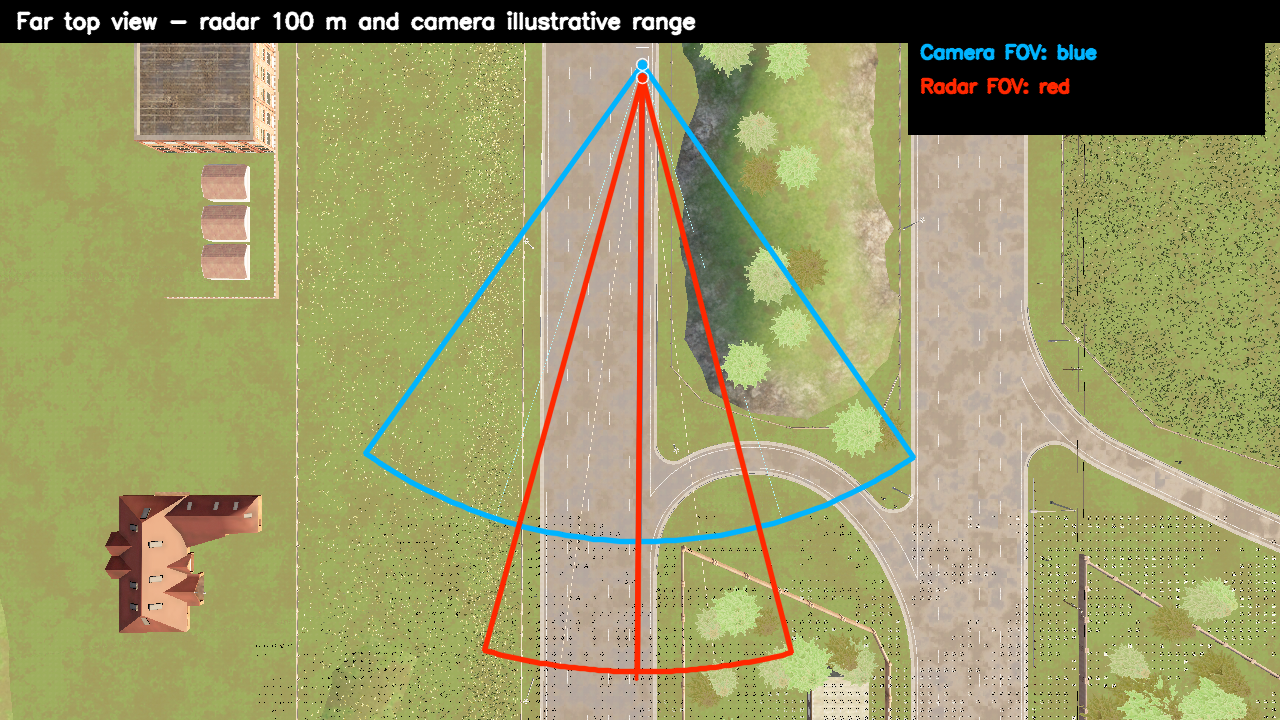
\includegraphics[width=\columnwidth]{../../report/assets/evidence/sensor_far_top_view.png}
  \caption{Top-view sensor coverage in the CARLA ego vehicle. The camera
  supplies vehicle confirmation; radar supplies range and relative velocity.}
  \label{fig:architecture}
\end{figure}

The camera stream is processed by a YOLO26n model fine-tuned for the single
\textit{car} class. The final dataset contains 1,505/300/200 train/validation/
test images with 1,872/379/264 boxes. Training at $640\times640$ for 100 epochs
produced precision 0.9919, recall 0.9642, $\mathrm{mAP}_{50}$ 0.9940, and
$\mathrm{mAP}_{50:95}$ 0.9495 at the best epoch. Ground truth is used only
offline to generate labels; it is not available to the online AEB decision.

Fig.~\ref{fig:yolo_training} summarizes the final training run. The model is
used conservatively: it supplies an image-space class check for a target already
selected by radar, rather than a stand-alone collision decision. This division
keeps the velocity-sensitive risk calculation tied to radar quantities while
still rejecting a radar target that is not visually associated with a vehicle.

\begin{figure}[t]
  \centering
  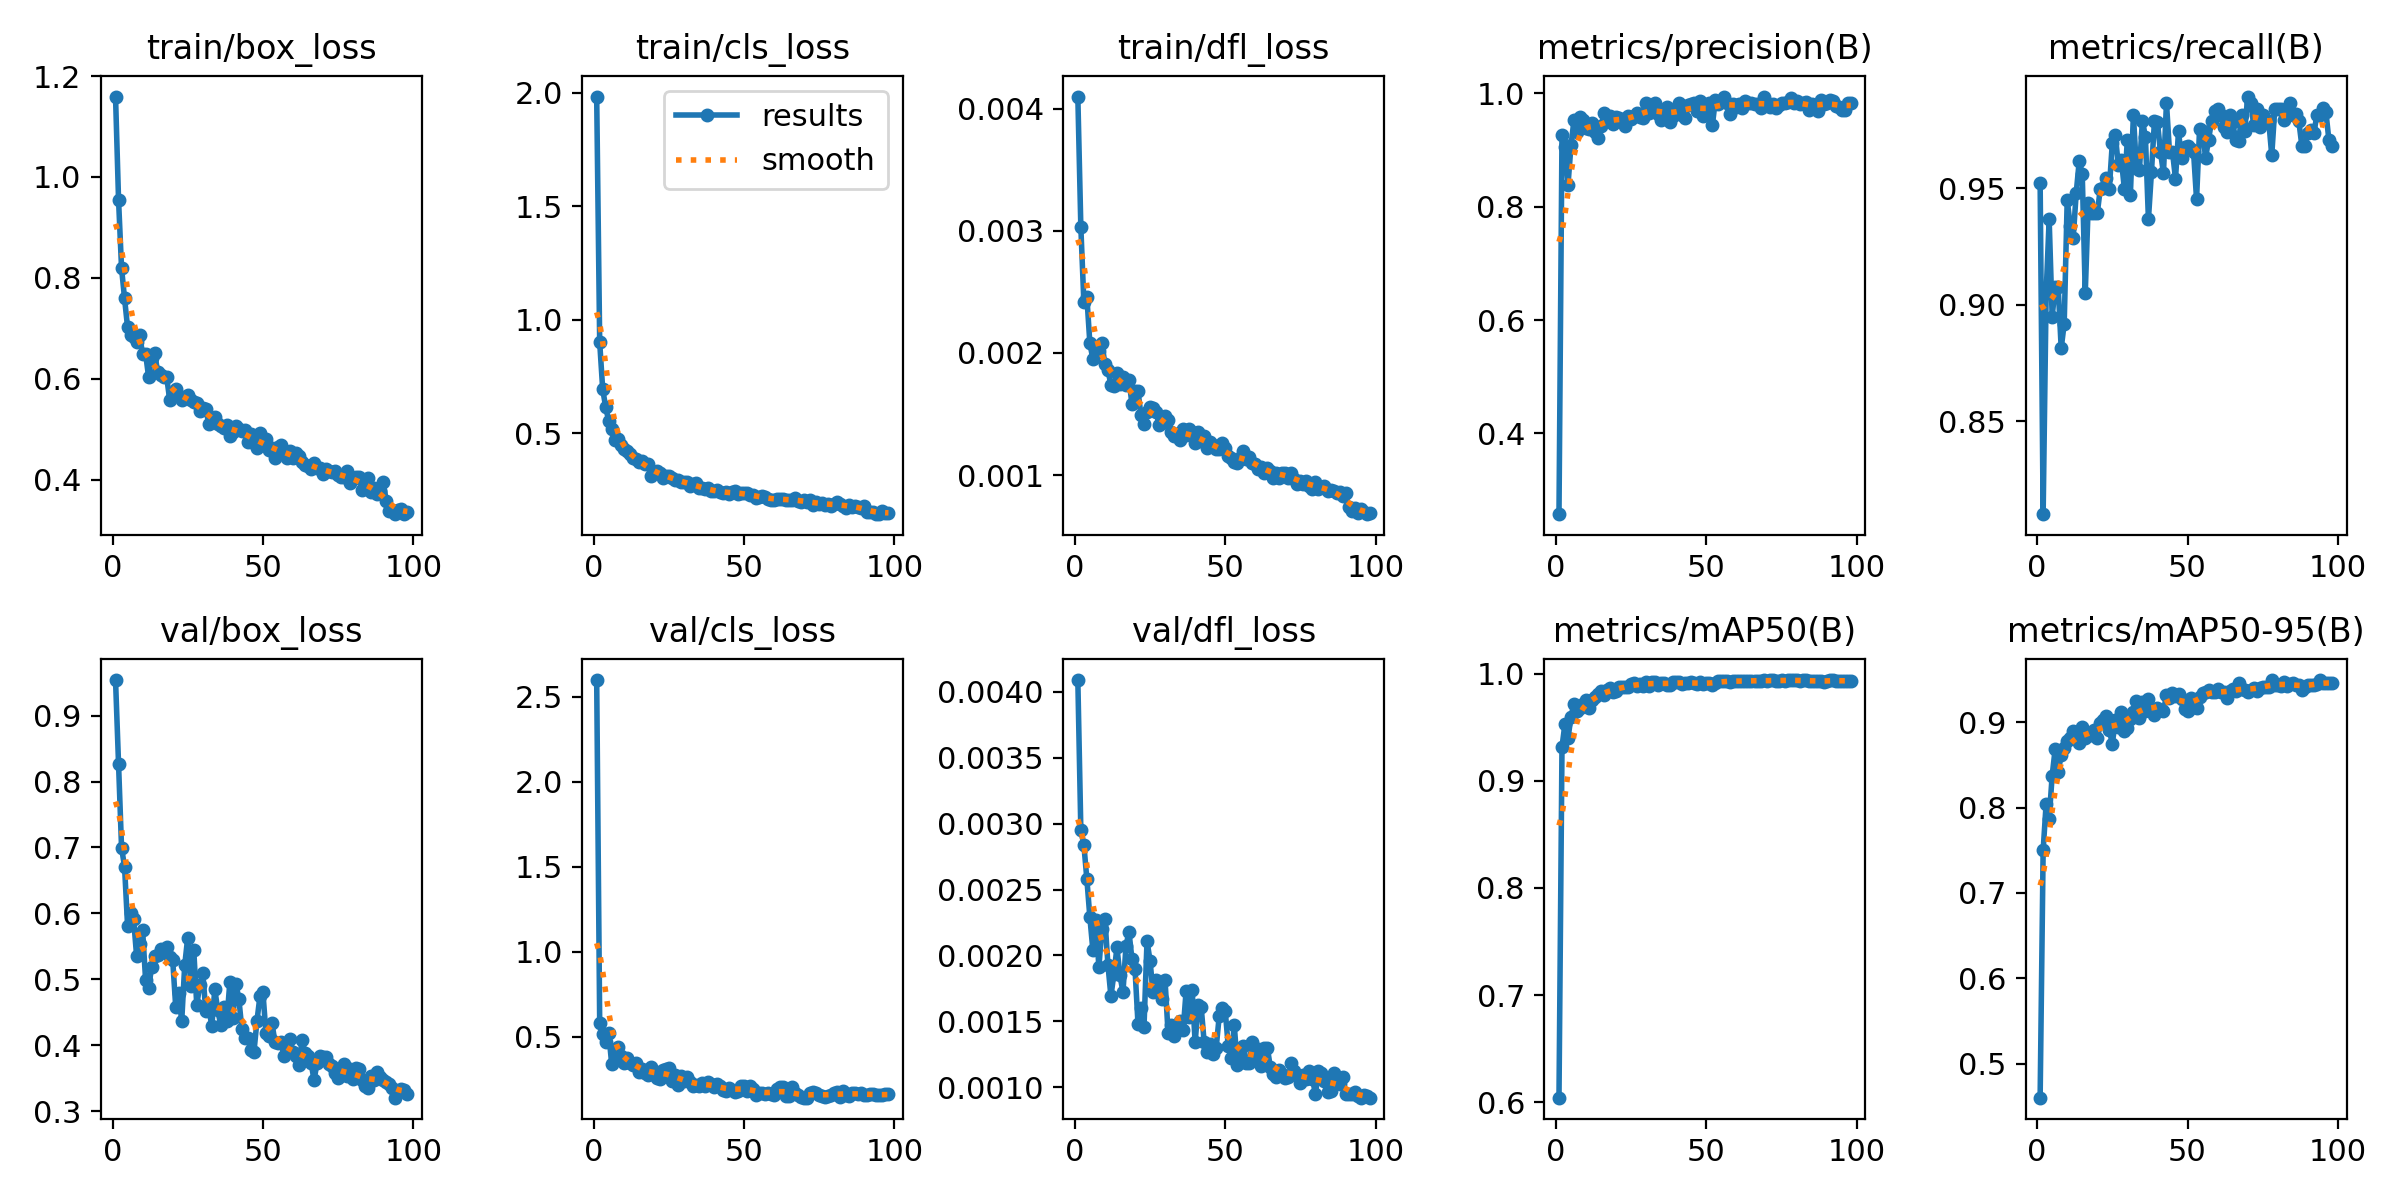
\includegraphics[width=\columnwidth]{../../report/assets/evidence/yolo_training_results.png}
  \caption{Training curves of the YOLO26n model used for camera verification.}
  \label{fig:yolo_training}
\end{figure}

\subsection{Object-Level Radar Processing}
A single radar return is not allowed to trigger braking. Returns first pass a
region-of-interest test: they must lie ahead of the ego vehicle, within the
configured range and height limits, and near the predicted ego path. Remaining
returns are connected into clusters when their planar separation, vertical
separation, and relative-velocity difference are sufficiently small. The
representative longitudinal coordinate is the 20th percentile of a cluster,
which avoids letting returns from the rear of a vehicle push the estimated
obstacle farther away. Lateral position, height, and relative velocity use
medians instead.

The cluster tracker predicts longitudinal position with relative velocity and
associates the next measurement by position and velocity. A track becomes
confirmed after three consecutive hits; lost tracks are released after the
configured miss limit. This produces a small object list with distance, lateral
offset, relative velocity, point support, and track age. The design is not a
radar signal-processing model or a probabilistic tracker; it is an explicit
object layer placed between CARLA radar returns and the AEB decision.

This object abstraction also makes the decision traceable. The target selector
considers only confirmed, non-stale tracks. It first prefers the smallest finite
TTC and uses longitudinal distance to break a tie. Hence a lateral reflection or
a one-frame point cannot directly override vehicle control. The track confidence
used in the user interface is only a deterministic proxy based on point support,
recent hits, and freshness; it is not radar cross section, signal-to-noise ratio,
or a calibrated existence probability. This distinction matters because CARLA
does not expose the raw FMCW signal-processing chain represented by production
automotive radar.

\subsection{Path-Aware Target Selection}
The nearest object is not necessarily collision-relevant. A constant-curvature
path is estimated from ego speed, yaw rate, and steering input. Its horizon is
the smaller of the 100-m radar range and a speed-dependent look-ahead distance.
Each confirmed object is compared with this path, and objects outside the
lateral corridor are rejected before risk evaluation. The remaining candidates
are ordered by finite TTC and then longitudinal distance. A selected target must
also remain stable for five frames, except when a short-distance or strongly
negative stopping-margin condition requires immediate braking. This additional
gate separates a persistent lead vehicle from a transient return.

The path representation estimates relevance, not a collision-free trajectory or
a lane map. When curvature is close to zero, the path is a straight line;
otherwise a point at arc length $s$ follows
\begin{equation}
x(s)=\frac{\sin(\kappa s)}{\kappa},\qquad
y(s)=\frac{1-\cos(\kappa s)}{\kappa}.
\label{eq:path}
\end{equation}
The closest distance from a radar object to the sampled curve is compared with
the lateral AEB limit. This keeps the method independent of CARLA actor identity
and lane labels, while making its intended behavior on curves and adjacent
traffic inspectable in the logs.

\subsection{Camera Verification}
For a radar point transformed to camera coordinates $(X_c,Y_c,Z_c)$, its pixel
coordinates are
\begin{equation}
 u=f_xX_c/Z_c+c_x,\qquad v=f_yY_c/Z_c+c_y, \quad Z_c>0,
 \label{eq:projection}
\end{equation}
where the focal length follows $f=W/[2\tan(\mathrm{FOV}/2)]$. A selected radar
object is camera-confirmed if its projected point lies inside a
non-maximum-suppressed YOLO car box. A 0.35-s confirmation hold absorbs
camera--radar timing differences. Radar remains the source of range and relative
velocity, while the camera prevents an unconfirmed radar target from initiating
braking. In particular, the camera does not estimate range or relative velocity,
and this late geometric gate is not presented as joint radar--camera tracking.

At each tick, a radar decision outside the supervisory `BRAKE' state passes
unchanged. If radar requests `BRAKE', the gate permits it only when the selected
target is currently inside a valid vehicle box or was confirmed within the
0.35-s hold window. Otherwise the decision is converted to `RELEASE' with zero
brake. The hold avoids a rapidly toggling command when camera, radar, and YOLO
arrive on different frames. It also exposes an important trade-off: a missed
camera detection can delay braking, which is treated as a limitation rather than
hidden by a radar-only fallback in the evaluated configuration.

\subsection{Risk Assessment and Staged PID Braking}
The predicted path is a constant-curvature curve estimated from ego yaw rate and
steering. Objects outside its lateral corridor are rejected. For a target at
distance $d$ with relative velocity $v_r$, closing speed and TTC are
\begin{equation}
 v_c=-v_r,\qquad \mathrm{TTC}=d/v_c \quad (v_c>0).
 \label{eq:ttc}
\end{equation}
TTC is infinite for a non-closing target. The required stopping distance is
\begin{equation}
 d_\mathrm{req}=\max\left(d_0,v_e t_r+\frac{v_e^2}{2a_e}
 -\frac{v_t^2}{2a_t}+d_0\right),
 \label{eq:stopping}
\end{equation}
where $v_e,v_t$ are ego and target speeds, $t_r$ is response time, $a_e,a_t$
are assumed emergency decelerations, and $d_0$ is a safety offset.

The controller uses both time-based and distance-based risk because neither is
sufficient alone. TTC is not a hazard measure for a target moving away, whereas
stopping distance accounts for ego speed, assumed response delay, and the
target's own ability to decelerate. The distance margin is
\begin{equation}
m_d=d-d_\mathrm{req}.
\label{eq:margin}
\end{equation}
An active `BRAKE' state is therefore requested either by a low TTC or by an
insufficient margin. The PID input combines a positive margin deficit with a
positive TTC deficit. Its integral is clamped, the derivative is used only when
error is increasing, and the output is rate-limited. These choices avoid a large
release--reapply oscillation in discrete 20-Hz control; they do not claim an
optimal vehicle-braking controller.

The supervisory state machine contains `NORMAL', `WARNING', `BRAKE', and
`RELEASE'. Soft, medium, hard, and emergency are brake-command schedules inside
`BRAKE', rather than four independent states. The controller enters `BRAKE' from
TTC or stopping-margin risk. Within it, the PID command is rate-limited and
clipped to the applicable brake interval. This retains a continuous command
while allowing immediate maximum braking in an emergency.

\section{Experimental Setup}
The simulator runs synchronously at 20 Hz in Town04 under ideal weather. The ego
vehicle is a Tesla Model 3 with a windshield RGB camera and a bumper-mounted
forward radar. A hazardous scenario passes when AEB brakes without collision;
a non-hazardous scenario passes only if it produces no false brake. Logged
metrics include collision status, minimum gap, first-brake distance, ego speed,
TTC, and brake command.

\begin{table}[t]
\caption{Key simulator and controller parameters.}
\label{tab:config}
\centering
\footnotesize
\begin{tabular}{p{0.46\columnwidth}r}
\toprule
Parameter & Value \\
\midrule
RGB camera / horizontal FOV / tick & 1280$\times$720 / 70$^\circ$ / 0.05 s \\
Radar range / horizontal--vertical FOV & 100 m / 30$^\circ$--6$^\circ$ \\
Radar points per second / tick & 2000 / 0.05 s \\
Track confirmation / target confirmation & 3 / 5 frames \\
Warning / brake TTC & 3.0 / 1.5 s \\
Response time / ego deceleration & 0.20 s / 8.0 m/s$^2$ \\
Staged brake: soft / medium / hard / emergency & 0.55 / 0.75 / 0.90 / 1.00 \\
\bottomrule
\end{tabular}
\end{table}

The final evidence suite contains CCR stationary (CCRs), moving (CCRm), and
braking (CCRb) cases plus clear-road, adjacent-lane, curve, cut-in, cut-out,
and multi-actor cases. Table~\ref{tab:scope} separates the intended ODD from
stress tests. This avoids interpreting a single aggregate pass rate as an
unconditional safety claim.

The final suite uses the YOLO ONNX model, the radar-object pipeline, geometric
camera verification, and the staged-PID configuration. A hazardous case passes
only when no collision is reported; a non-hazardous case passes only when the
system does not brake unnecessarily. The fixed-tick logs, rather than display
frame rate or video playback, provide the quantitative evidence. The suite is
deterministic in the simulator and is used to map behavior in configured cases,
not to estimate statistical reliability.

The scenario groups have separate purposes. CCRs tests a stationary lead vehicle
that stays relevant throughout the run. CCRm tests a slower lead vehicle, so the
closing speed can be much smaller than ego speed. CCRb introduces a lead vehicle
that brakes after both vehicles are moving. Cut-in and cut-out test changes in
path relevance, while adjacent-lane, curve, and multi-actor cases exercise the
ability to ignore a nearby but non-relevant object. This family-based setup is
inspired by car-to-car evaluation structures, but it does not reproduce the full
test apparatus, measurements, or certification conditions of Euro NCAP.

\begin{table}[t]
\caption{Evaluation scope and interpretation.}
\label{tab:scope}
\centering
\footnotesize
\begin{tabular}{p{0.20\columnwidth}p{0.34\columnwidth}p{0.31\columnwidth}}
\toprule
Set & Typical conditions & Purpose \\
\midrule
Designed ODD & Highway, cars only, ideal weather, mainly 50--80 km/h & Verify target operating range \\
Stress tests & 95--110 km/h, short gaps, hard braking, difficult cut-in & Identify operating limits \\
\bottomrule
\end{tabular}
\end{table}

\section{Results and Discussion}
\subsection{Overall Outcomes}
Table~\ref{tab:results} reports the final staged-PID, camera--radar system.
All 38 cases in the designed ODD pass. The full suite contains 63 passes among
66 cases. The three collisions are retained: CCRb at 95 and 110 km/h with a
20-m initial gap, and a 100/60-km/h cut-in with a 25-m initial gap. They reveal
that, once the lead vehicle brakes or enters the ego corridor late, the available
perception and stopping time becomes insufficient.

\begin{table}[t]
\caption{Final result with camera--radar fusion and staged PID.}
\label{tab:results}
\centering
\footnotesize
\begin{tabular}{lrrr}
\toprule
Evaluation set & Cases & Pass & Fail \\
\midrule
Designed ODD & 38 & 38 & 0 \\
Stress / limit finding & 28 & 25 & 3 \\
\midrule
Total & 66 & 63 & 3 \\
\bottomrule
\end{tabular}
\end{table}

\begin{table}[t]
\caption{CCRb sweep: P = pass and C = collision.}
\label{tab:ccrb_sweep}
\centering
\footnotesize
\begin{tabular}{c*{6}{c}}
\toprule
Ego speed / gap & 20 m & 30 m & 40 m & 50 m & 60 m & 80 m \\
\midrule
50 km/h  & P & P & P & P & P & P \\
65 km/h  & P & P & P & P & P & P \\
80 km/h  & P & P & P & P & P & P \\
95 km/h  & C & P & P & P & P & P \\
110 km/h & C & P & P & P & P & P \\
\bottomrule
\end{tabular}
\end{table}

\subsection{Behavior Across Scenario Families}
The stationary, moving, braking, and cut-in families reveal different forms of
risk. For CCRm, absolute ego speed alone is not decisive: the 110/80-km/h,
20-m case passes because its closing speed is about 30 km/h. By contrast, a
stationary lead vehicle or a braking lead vehicle can remove closing-speed margin
quickly. The configured clear-road, adjacent-lane, curved-road, and multi-actor
cases provide complementary checks: no unnecessary braking was observed for the
specified adjacent-lane and curved-road cases, while same-lane hazards still
triggered braking. These are configured-case observations, not an ablation that
attributes a quantitative reduction in false brakes to a single component.

The representative values illustrate the same point. In the 80/50-km/h CCRm
case, braking begins at a gap of 18.97 m and the smallest measured gap is
14.45 m. In the 110/80-km/h CCRm case, braking starts at 18.96 m and the minimum
gap is 15.01 m. Both are different from the CCRb cases even though some initial
gaps are identical, because the leading vehicle continues moving instead of
removing its speed. The result motivates retaining relative velocity and stopping
margin in the controller rather than using a fixed distance threshold.

\subsection{Observed Failure Boundaries}
Fig.~\ref{fig:ccrb} contrasts a successful 80-km/h CCRb case with its 95-km/h
limit case. At 80 km/h and a 20-m initial gap, braking begins at 18.56 m and the
minimum gap remains 1.96 m. At 95 km/h under the same gap, the controller still
commands braking but collision occurs with a 0.013-m minimum gap. Likewise, the
100/60-km/h cut-in is detected only after the entering vehicle reaches the ego
corridor, so braking begins at 7.26 m and is too late to avoid contact.

\begin{figure}[t]
  \centering
  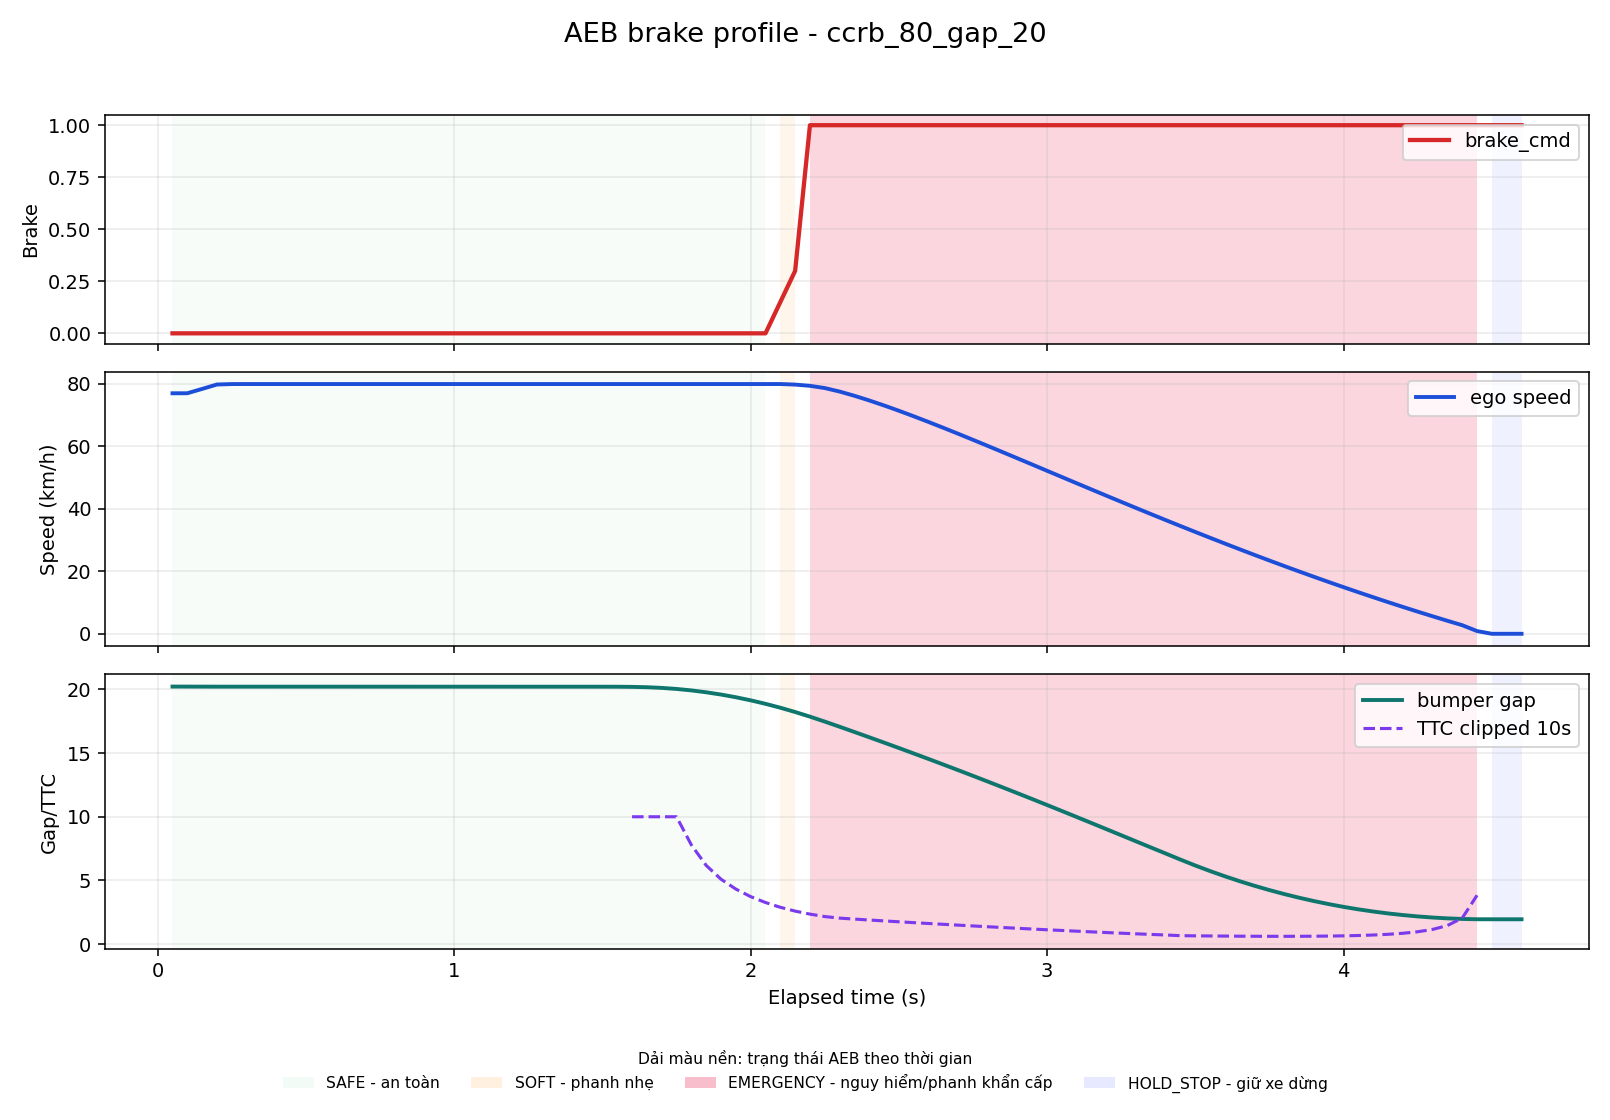
\includegraphics[width=0.49\columnwidth]{../../report/assets/evidence/brake_profile_ccrb_80_gap_20.png}
  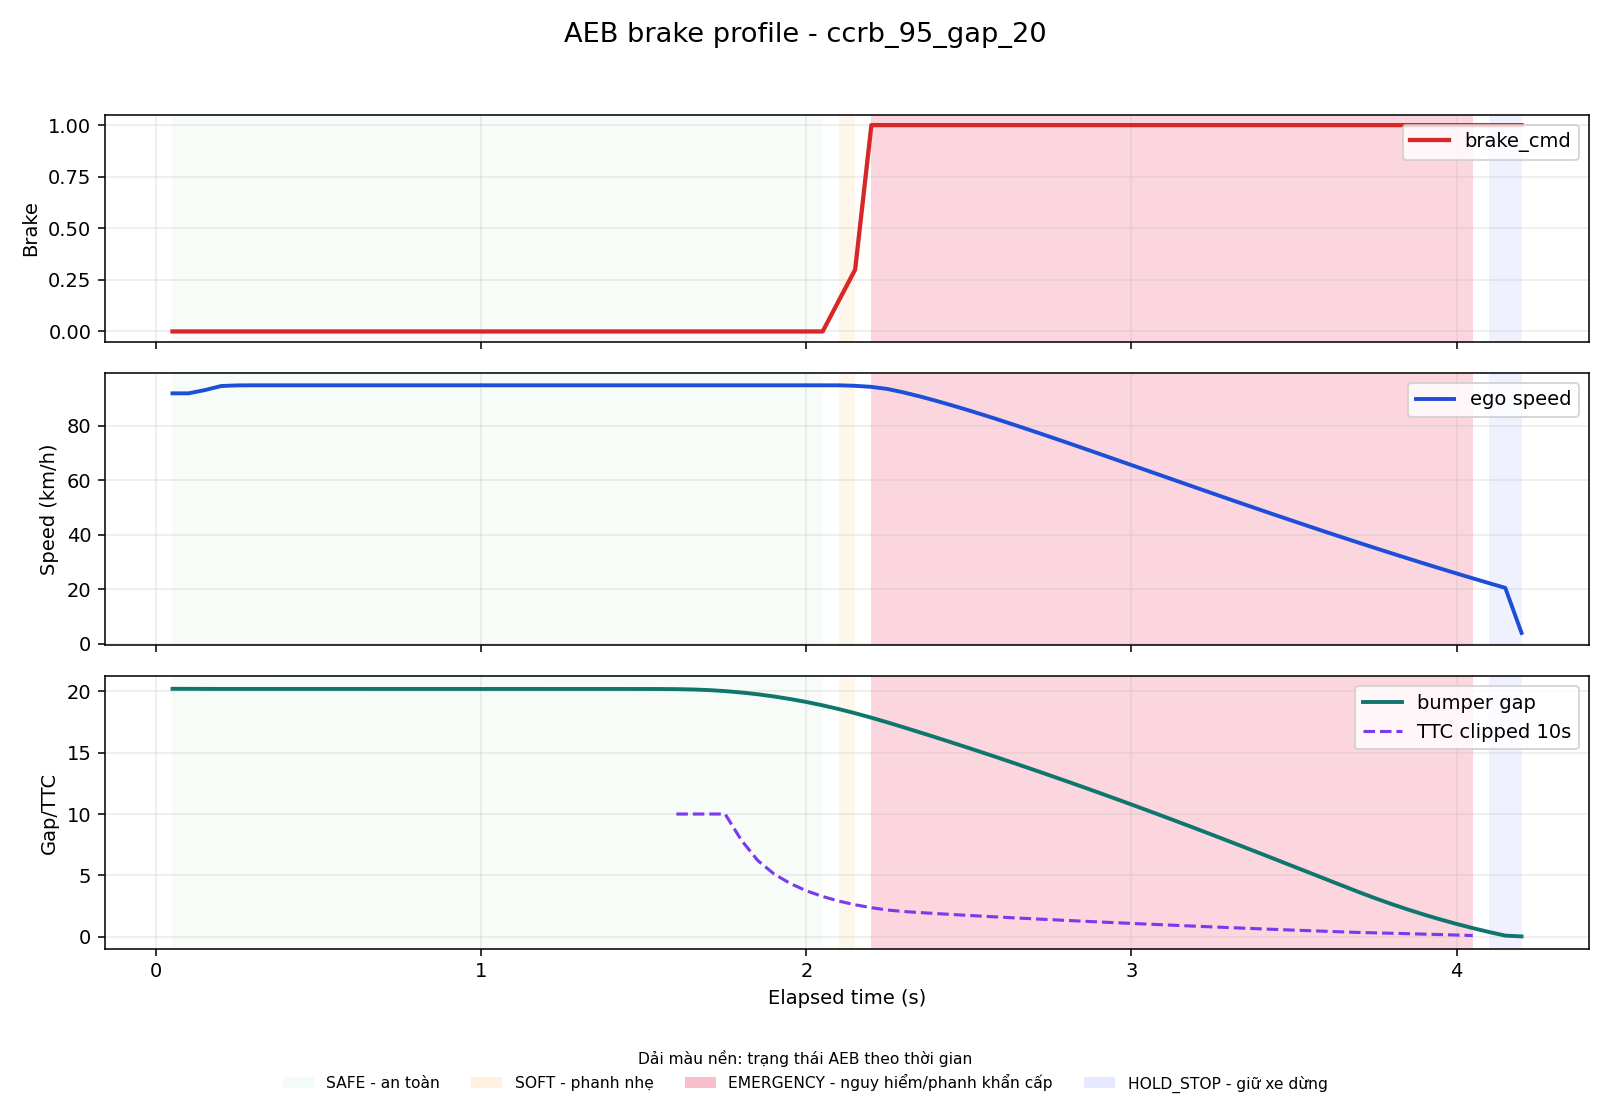
\includegraphics[width=0.49\columnwidth]{../../report/assets/evidence/brake_profile_ccrb_95_gap_20.png}
  \caption{Brake profiles for CCRb at a 20-m initial gap: pass at 80 km/h
  (left) and collision at 95 km/h (right).}
  \label{fig:ccrb}
\end{figure}

\begin{table*}[t]
\caption{Representative final-evidence scenarios. Brake quantities are sampled
at the first nonzero brake command.}
\label{tab:representative}
\centering
\footnotesize
\begin{tabular}{llrrrr}
\toprule
Family & Scenario & Result & Brake speed (km/h) & Brake gap (m) & Minimum gap (m) \\
\midrule
CCRs & ccrs\_80 & Pass & 69.72 & 32.12 & 7.70 \\
CCRm & ccrm\_110\_80\_gap\_20 & Pass & 108.00 & 18.96 & 15.01 \\
CCRb & ccrb\_80\_gap\_20 & Pass & 79.92 & 18.56 & 1.96 \\
CCRb & ccrb\_95\_gap\_20 & Collision & 94.90 & 18.56 & 0.013 \\
Cut-in & cutin\_80\_50\_gap\_25 & Pass & 79.92 & 10.46 & 5.51 \\
Cut-in & cutin\_100\_60\_gap\_25 & Collision & 99.90 & 7.26 & 0.476 \\
\bottomrule
\end{tabular}
\end{table*}

The CCRb sweep in Table~\ref{tab:ccrb_sweep} makes the stopping-distance boundary
visible: the 20-m initial gap passes at 80 km/h but collides at 95 and 110 km/h,
whereas the reported larger gaps pass. The evidence does not show that perception
failed in those cases; the final controller still commands braking. It supports a
more limited conclusion: in this configured braking scenario, the available
distance becomes insufficient as speed increases. The cut-in failure has a
different mechanism. The target begins outside the ego corridor, so it becomes
relevant only after entering that corridor. At 100/60 km/h with a 25-m initial
gap, confirmation and braking begin at 7.26 m, leaving too little distance.
Table~\ref{tab:representative} places these observations alongside two successful
cases. Its values reinforce that the result should not be read as a single speed
threshold: distance, target motion, and when a vehicle becomes path-relevant all
affect the remaining stopping margin.

The late-fusion gate has a deliberate asymmetry. Radar can establish that an
object is closing and within the predicted path, but the gate still requires a
recent image-space vehicle match before allowing a brake command. This reduces
the chance that an unclassified return alone becomes a braking target in the
configured adjacent-lane cases. The corresponding cost is visible in cut-in:
when a vehicle crosses into the ego corridor late, the first relevant radar
object and the first usable camera confirmation are both delayed. The 80/50-km/h
case retains enough distance after braking; the 100/60-km/h case does not.

\begin{figure}[t]
  \centering
  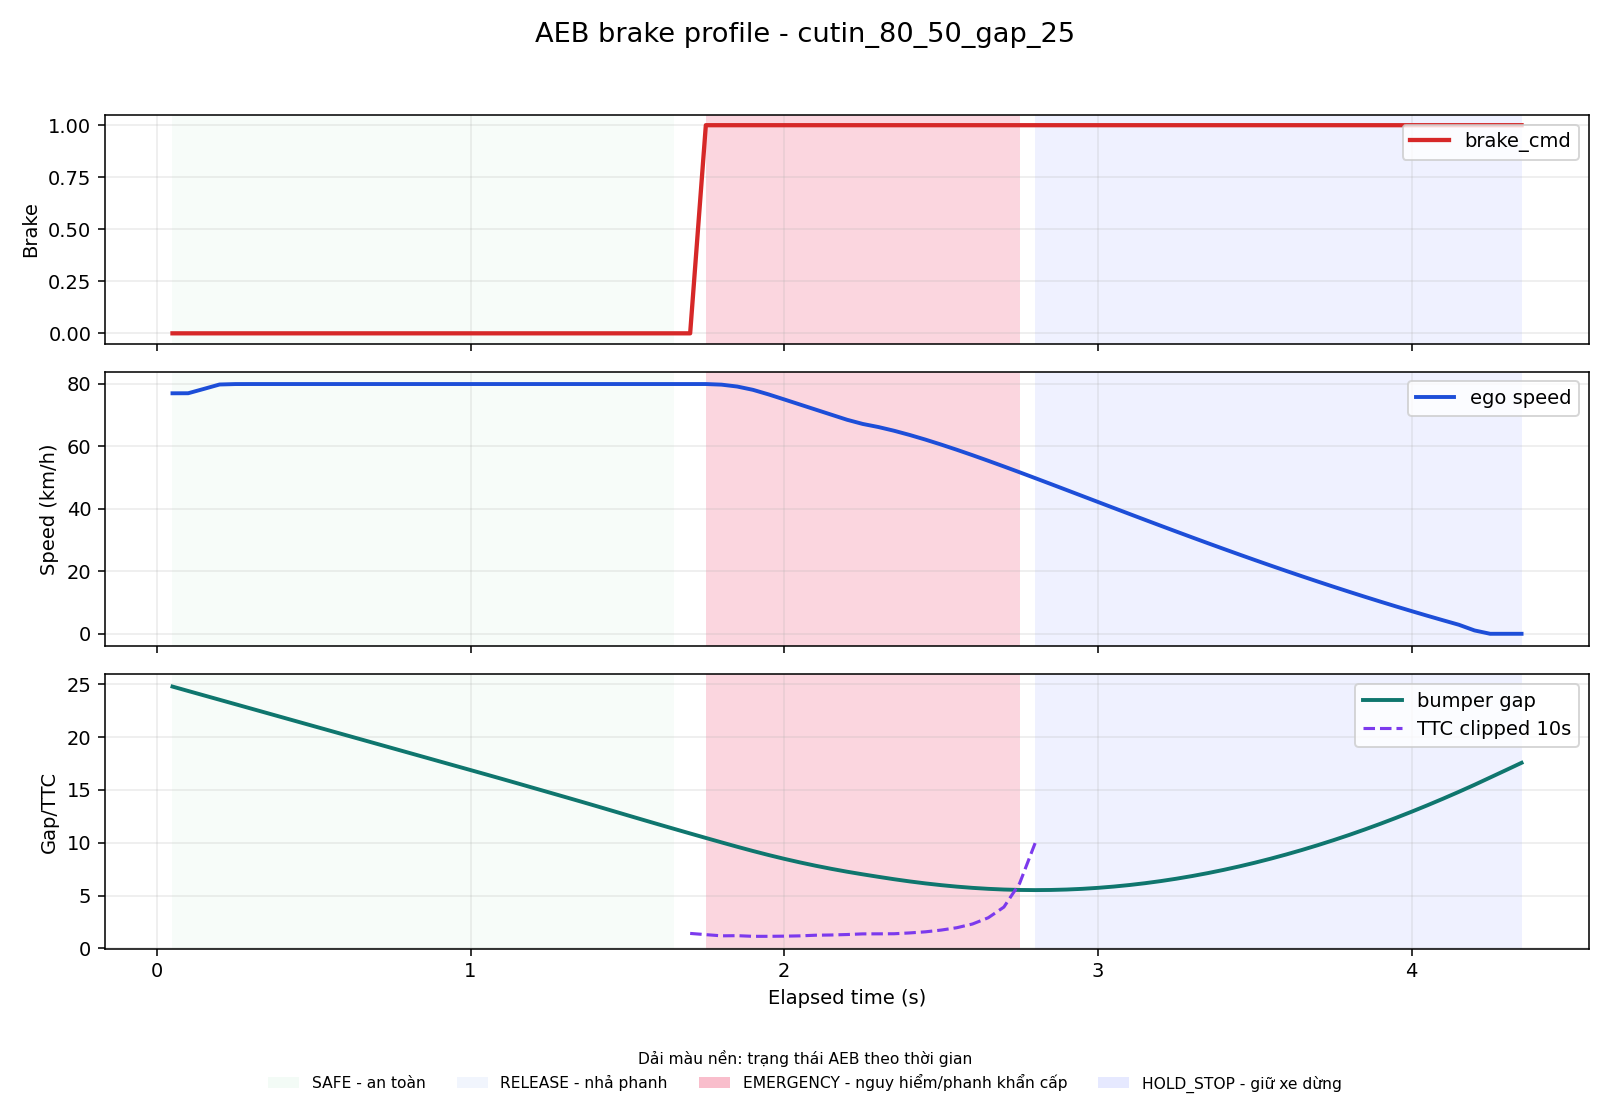
\includegraphics[width=0.49\columnwidth]{../../report/assets/evidence/brake_profile_cutin_80_50_gap_25.png}
  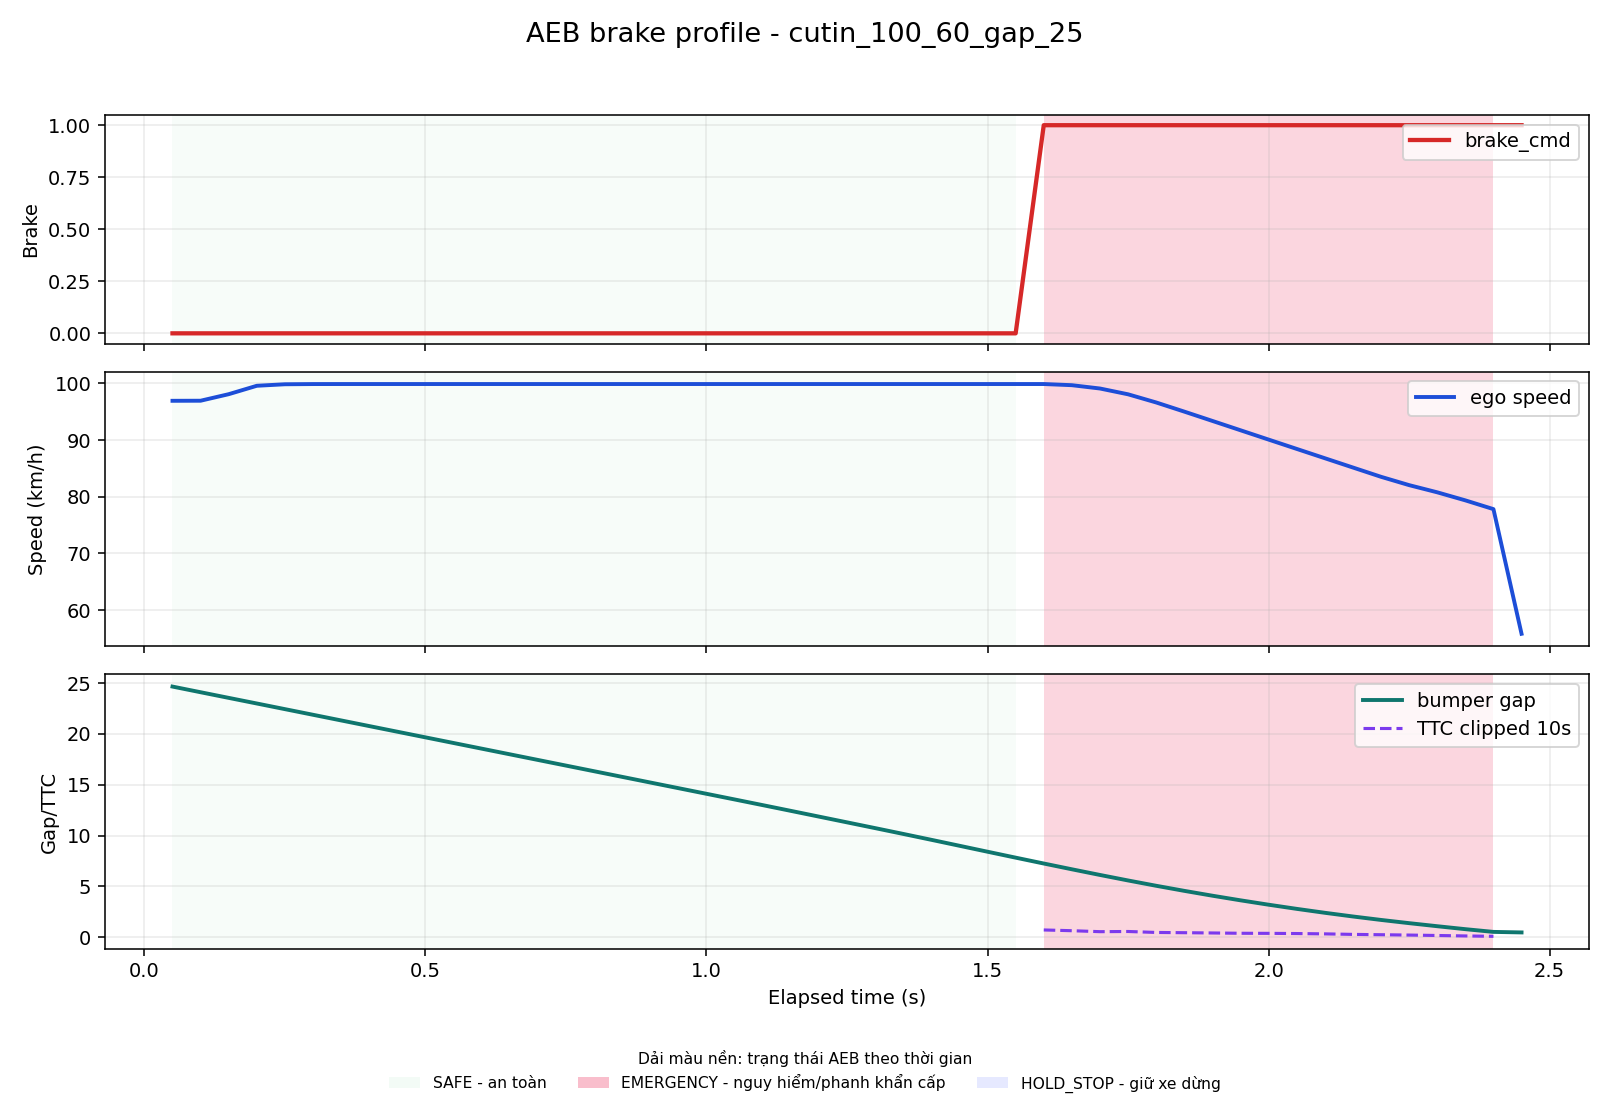
\includegraphics[width=0.49\columnwidth]{../../report/assets/evidence/brake_profile_cutin_100_60_gap_25.png}
  \caption{Cut-in brake profiles at a 25-m initial gap: pass at 80/50 km/h
  (left) and collision at 100/60 km/h (right).}
  \label{fig:cutin}
\end{figure}

This observation should not be generalized into a claim that camera verification
is always beneficial or that the configured path corridor is optimal. The final
evidence contains no repeated radar-only versus camera-gated comparison. It
instead documents a transparent behavior: a selected radar target must remain
kinematically relevant and visually confirmed, and the available margin can be
exhausted if that relevance appears late. A future estimator could combine
lateral motion, predicted lane entry, and uncertainty-aware association, but
would need its own controlled evaluation.

The controller outcome is also best interpreted through the stopping model. The
configured ego deceleration is 8.0 m/s$^2$ and the response term is 0.20 s, but
these are risk-model parameters inside CARLA rather than measurements of a
brake system. When a target is moving, the model subtracts its estimated stopping
distance; this is why a moderate-closing-speed CCRm case can retain a large
minimum gap even at high ego speed. When a CCRb target begins braking, its future
speed changes faster than a constant-relative-velocity TTC picture. The margin
and staged emergency limits provide an additional trigger, but neither can create
physical distance after the target becomes relevant. The boundary cases show
where the configured chain of perception, decision, and actuation runs out of
time.

The evidence also separates visualization from measurement. The graphical user
interface displays radar points, selected objects, YOLO boxes, target status,
TTC, and brake command, but the evaluation relies on synchronous simulation
ticks and generated logs. Video frame rate can differ from the 20-Hz simulator
tick and is not used as evidence for response time. Similarly, raw jerk derived
from CARLA state is retained for internal controller comparison but is not
interpreted as an on-road ride-comfort value. This separation keeps the paper
focused on outcomes that the project records consistently across the final suite.

\section{Limitations}
The findings are limited to CARLA 0.9.11, Town04, ideal weather, and car-to-car
scenarios. CARLA radar supplies simulated detections rather than a raw FMCW
signal chain, and the YOLO dataset is concentrated in the same simulation domain.
The camera gate can withhold a brake if a detection is missed or calibration is
misaligned. No randomized repeated trials or quantitative radar-only/fusion
ablations are available in the final evidence, so the study does not estimate
variance or compare alternatives statistically. Pedestrians, motorcycles,
adverse weather, actuator delay, tire-road interaction, and full ABS dynamics
are outside the evaluated scope. These limitations identify the next validation
steps; they do not turn the simulated result into a vehicle-safety claim.

The most direct extensions are repeated trials with controlled seeds, explicit
radar-only and camera-gated baselines, and reporting of collision, minimum gap,
and unnecessary-brake distributions. A second group of extensions concerns the
late cut-in boundary: lateral-motion prediction and time-to-lane-entry estimates
could make an entering vehicle relevant before it occupies the center of the
ego corridor. Neither follows automatically from widening the corridor, because
that would also increase exposure to adjacent-lane false targets. A more realistic
evaluation would also need diverse maps, lighting and weather, pedestrians and
two-wheelers, actuator delay, and tire-road dynamics.

The detector result is also domain-limited. YOLO26n was fine-tuned with
CARLA-derived labels for one `car' class, mainly in Town04 and favorable visual
conditions. Its validation precision, recall, and mAP support that narrow
verification role, but they do not establish transfer to another map, night,
rain, pedestrian targets, or camera hardware. The radar-side filters are equally
configuration-dependent: their range, height, and lateral thresholds were chosen
for the present vehicle and highway scenarios. Publishing these parameters and
the exact scenario split is consequently more useful than presenting the result
as a general AEB performance number.

\section{Conclusion}
This paper presented a CARLA AEB system that fuses object-level radar processing
with YOLO vehicle confirmation, path-aware target selection, TTC and stopping
distance, and staged PID braking. It passes 38/38 cases in the stated ODD and
63/66 cases in the complete limit-finding suite. The retained failures define
the current high-speed, short-gap, and late cut-in limitations. Future work will
add repeated-seed ablation studies, diverse weather and maps, probabilistic
multi-object fusion, and vehicle/actuator dynamics before any real-world claim.

\balance
\bibliographystyle{IEEEtran}
\bibliography{references}
\end{document}
